\subsection{Lexer et Parseur}

\begin{frame}{Lexer}
    
    \hspace{-5mm}

    \begin{block}{La création}
        \begin{itemize}
            \item Définition d'expressions régulières pour certains jetons :
            \begin{itemize}
                \item DIGIT [0-9] 
                \item IDENT [a-zA-Z][a-zA-Z0-9\_]*
            \end{itemize}
            \item Création de jetons pour les symbôles terminaux $\longrightarrow$ +, physical, system \dots
        \end{itemize}
    \end{block}
    
    \begin{block}{Jetons existants}
        \begin{itemize}
            \item Opérateurs binaires et unaires
            \item Littéraux
            \item Types de données et types de fonctions
            \item Jetons spécifiques à CHIPS
            \item Jetons existants dans d'autres langages
        \end{itemize}
    \end{block}
\end{frame}

\begin{frame}{Parseur}

    \hspace{-5mm}

    \begin{figure}
        \centering
        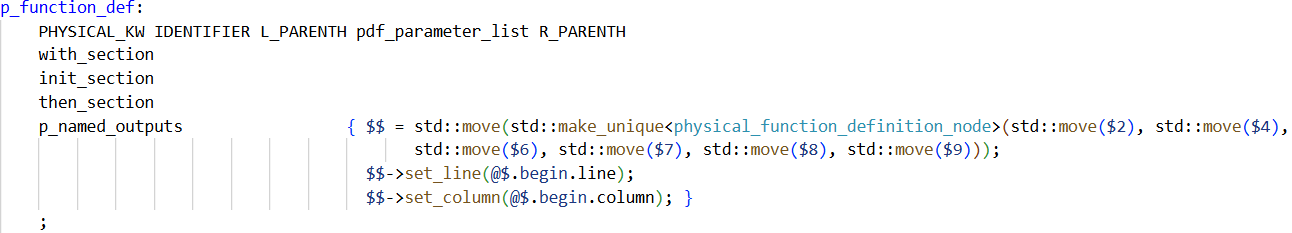
\includegraphics[width=\textwidth]{img/grammar.png}
        \caption{Exemple d'une règle de grammaire}
        \label{fig:grammaire_physical}
    \end{figure}
    
    \begin{block}{Fonctionnement}
        \begin{itemize}
            \item Déclaration des règles $\longrightarrow$ utilisation de jetons terminaux/non-terminaux
            \item Création des noeuds de l'AST
            \item Affectation du numéro de la ligne et la colonne $\longrightarrow$ pour les erreurs
        \end{itemize}
    \end{block}
\end{frame}


\subsection{Sérialisation vers XMI}

\begin{frame}{Passage de l'AST au modèle XMI}
    \begin{itemize}
        \item \textbf{Pourquoi le format XMI ? :}
        \begin{itemize}
            \item Standard de l'OMG pour l'échange de métadonnées.
            \item Interopérabilité avec \textbf{EMF} (Eclipse Modeling Framework).
        \end{itemize}
        \vfill
        \item \textbf{Qu'est-ce que le Méta-modèle CHIPS (Ecore) ? :}
        \begin{itemize}
            \item Définit la "grammaire" stricte du modèle (entités, relations).
            \item Utilisation des schémas \texttt{chips1.1.ecore} ou \texttt{chips2.ecore}.
        \end{itemize}
        \vfill
        \item \textbf{Comment valider le format ? :}
        \begin{itemize}
            \item Garantie de conformité via un script de validation basé sur EMF (\texttt{xmi\_validator.py}).
        \end{itemize}
    \end{itemize}
\end{frame}

\begin{frame}{Transformation et parcours de l'AST}
    \begin{columns}
        \begin{column}{0.6\textwidth}
            \begin{itemize}
                \item \textbf{ChipsToXmiVisitor :}
                \begin{itemize}
                    \item Parcours récursif de l'AST.
                    \item Génération dynamique du flux XML.
                \end{itemize}
                \item \textbf{Gestion du contexte :}
                \begin{itemize}
                    \item \texttt{m\_currentPath} : Maintien de la position hiérarchique (ex: \texttt{//@preamble/@definitions.0}).
                    \item Construction incrémentale des fragments d'URI.
                \end{itemize}
                \item \textbf{ChipsToXmiWriter :} Reprend la sortie du visiteur et sépare le corps du XMI (\texttt{bodywriter}) et les en-tête pour gérer dynamiquement les \textit{namespaces}.
            \end{itemize}
        \end{column}
        \begin{column}{0.4\textwidth}
            \centering
            \textbf{Flux de données}
            \vspace{0.5cm}
            \begin{exampleblock}{Pipeline}
                Code CHIPS \\
                $\downarrow$ \\
                AST (C++) \\
                $\downarrow$ \\
                \textbf{Visiteur XMI} \\
                $\downarrow$ \\
                Modèle XMI
            \end{exampleblock}
        \end{column}
    \end{columns}
\end{frame}

\begin{frame}{Résolution des liens et gestion des symboles}
    \begin{itemize}
        \item \textbf{Problématique :} Faire le lien entre un \textit{nom} (code source) et un \textit{chemin relatif} (XMI).
        \item \textbf{Solution :} Une table des symboles double.
        \begin{itemize}
            \item \texttt{m\_symbolTable} : Lie un identifiant à son chemin XMI définitif.
            \item \texttt{m\_definitionsTable} : Gère les variables locales (\texttt{with}, \texttt{init}, \texttt{then}).
        \end{itemize}
    \end{itemize}
\end{frame}

\begin{frame}[fragile]{Exemple de résolution 1/5}
  Voici la définition du sous-composant logique :
  \begin{figure}
        \centering
        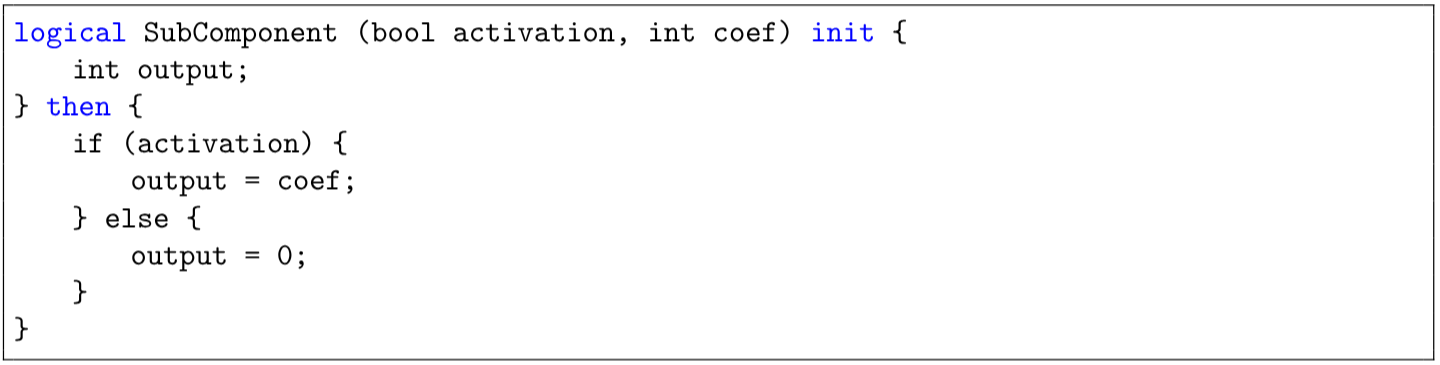
\includegraphics[width=\textwidth]{img/exemple_chips.png}
        \caption{Exemple d'un composant logique en CHIPS}
        \label{fig:logical_component}
    \end{figure}
\end{frame}

\begin{frame}[fragile]{Exemple de résolution 2/5}
    \begin{figure}
        \centering
        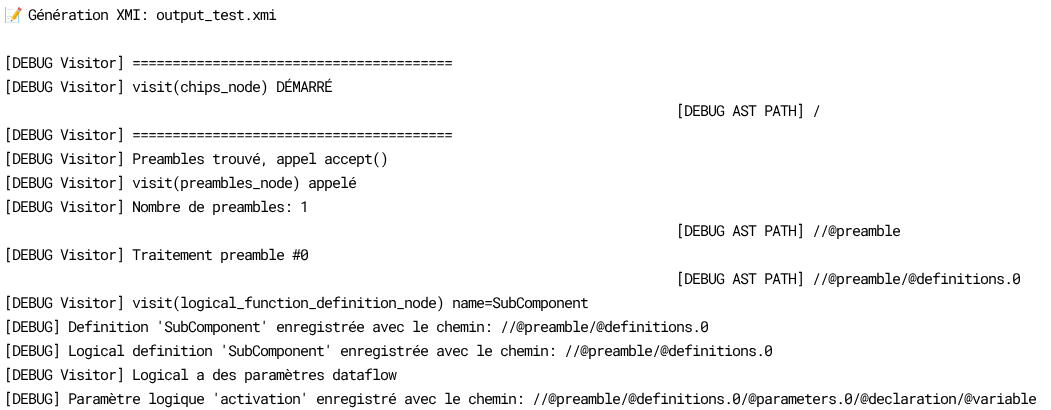
\includegraphics[width=\textwidth]{img/debug_message.png}
        \caption{Extrait des messages de debogage pour la génération XMI}
        \label{fig:xmi_debbug}
    \end{figure}
\end{frame}

\begin{frame}[fragile]{Exemple de résolution 3/5}
    \begin{figure}
        \centering
        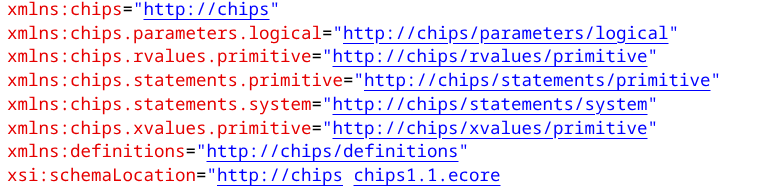
\includegraphics[width=\textwidth]{img/namespace.png}
        \caption{Extrait des namespaces générés}
        \label{fig:xmi_namespace}
    \end{figure}
\end{frame}

\begin{frame}[fragile]{Exemple de résolution 4/5}
  \begin{figure}
        \centering
        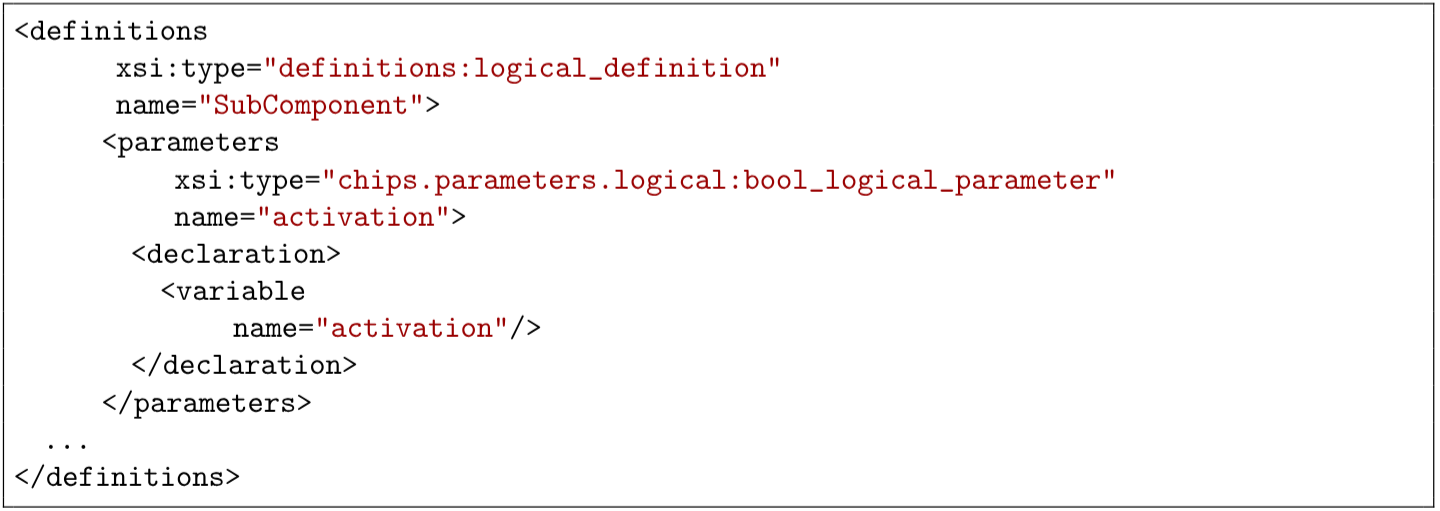
\includegraphics[width=\textwidth]{img/exemple_xmi.png}
        \caption{Extrait de la génération XMI du composant logique}
        \label{fig:xmi_writing}
    \end{figure}
\end{frame}

\begin{frame}[fragile]{Exemple de résolution 5/5}
  \begin{figure}
        \centering
        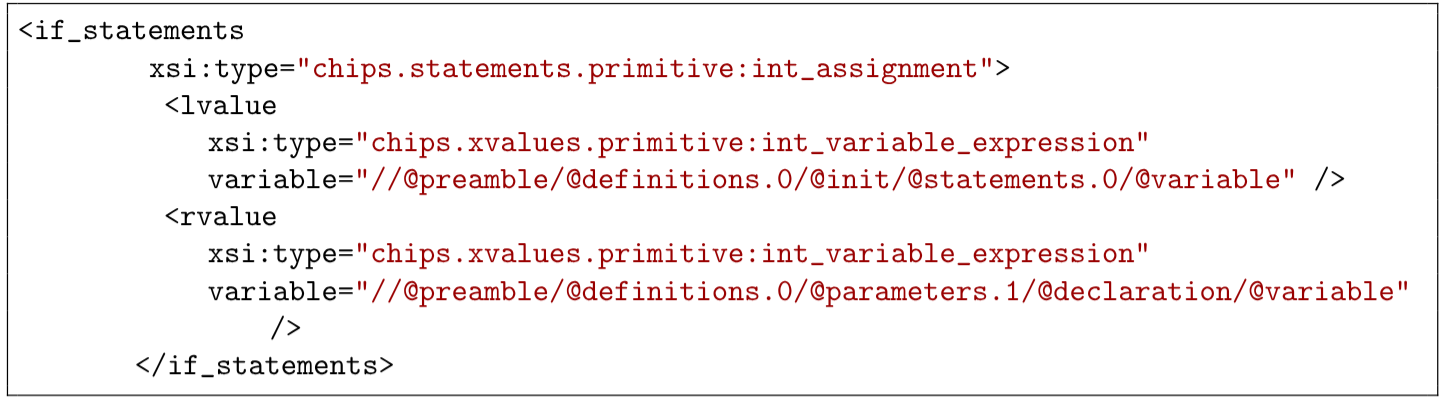
\includegraphics[width=\textwidth]{img/exemple_xmi_2.png}
        \caption{Extrait de la génération XMI du composant logique}
        \label{fig:xmi_writing_2}
    \end{figure}
\end{frame}